\section{Statistical Analysis}\label{sec:ciStat}

Statistical methods are used to distill two types of information from the collected dataset.
First, to determine the probability that the observed data is incompatible with the background-only (B-only) hypothesis.
Second, to determine the smallest putative signal such that, if extant, would produce a signal+background (S+B) hypothesis that is incompatible with the observed data.
The former is answered by a significance test, described in Section \ref{sec:ciSigTest}, while the latter is answered by setting a limit, described in Section \ref{sec:ciLimitSetting}.

\subsection{Likelihood Ratio and CLs Method}

\begin{figure}[h!]
\captionsetup[subfigure]{position=b}
\centering
\subfloat[][]{\label{fig:ciClsNobs}{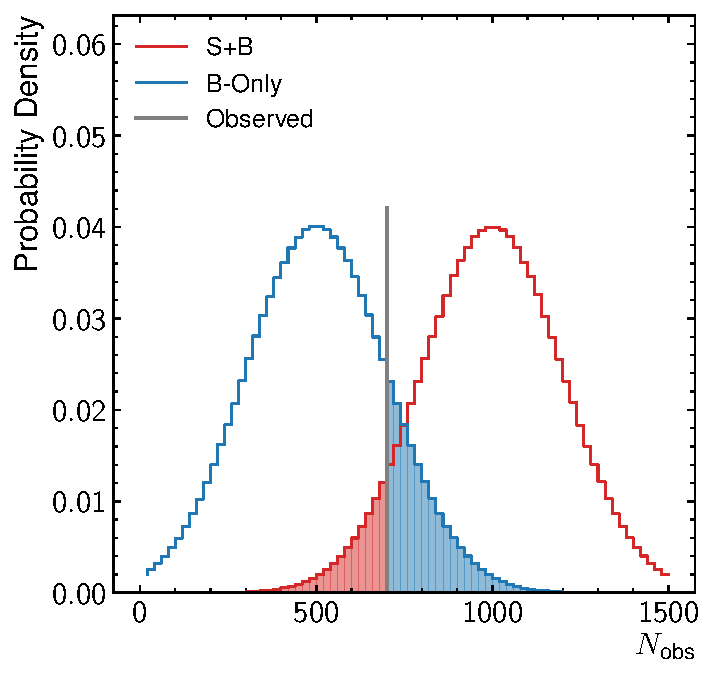
\includegraphics[width=0.5\textwidth]{figures/stats/stat-nobs.pdf}}}
\subfloat[][]{\label{fig:ciClsProfileLikelihood}{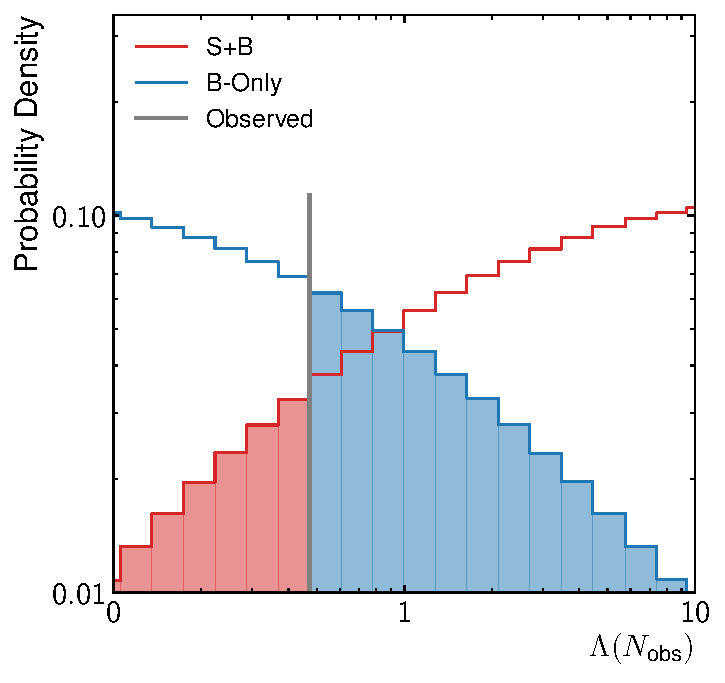
\includegraphics[width=0.5\textwidth]{figures/stats/stat-likel.pdf}}}
\caption{PDFs predicted by S+B and B-only hypotheses of test statistics (a) \nobs and (b) the likelihood ratio. Note the log scale of (b). In each case, the shaded regions mark the set of test statistic values for which each hypothesis would be more incompatible then with the observed value shown in grey.}
\label{fig:ciCls}
\end{figure}

% \begin{figure}[h!]
% \captionsetup[subfigure]{position=b}
% \centering
% 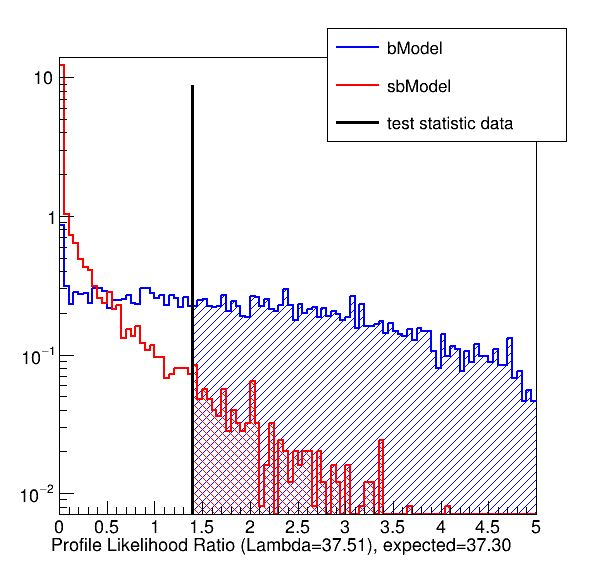
\includegraphics[width=0.5\textwidth]{figures/ci/profileLikelihoodPlots/toys-n29-fc-lambda-ll-const-LL-nToy5000-nSteps50-seed8.png}
% \caption{}
% \label{fig:ciClsProfileLikelihood}
% \end{figure}

% Test statistic: likelihood ratio
The fundamental tool used to compare two hypotheses is the \emph{test statistic}, a quantity calculated from the observed data.
Each hypothesis predicts a probability density function (PDF) that describes the probability to observe values of the test statistic.
The PDF of the B-only hypothesis, $\mathcal{L}(\nobs)$, is a function of the test statistic \nobs.
Composite hypotheses are more useful and are defined by additional parameters, $\theta$, that may be estimated from the observation.
In general, a B-only hypothesis defined by $\theta_0$ predicts a PDF of $\mathcal{L}(\nobs|\theta_0)$, while an S+B hypothesis defined by $\theta_1$ predicts a PDF of $\mathcal{L}(\nobs|\theta_1)$.
For example, a B-only hypothesis may predict a Gaussian PDF with a mean that is smaller than the average predicted by an S+B hypothesis.
An illustration is shown in Figure \ref{fig:ciClsNobs}.
Here, the B-only hypothesis is more compatible with an observation of \nobs=500 than \nobs=1,000, while the converse is true of the S+B hypothesis.
The choice to accept or reject a hypothesis is made by a comparison of their respective PDFs.

While the test statistic may be any quantity calculated from data, an optimal choice for the test statistic may be made to resolve the difference between the two hypotheses.
A common choice is to use the ratio of the S+B and B-only hypotheses to define the \emph{likelihood ratio} in Equation \ref{eqn:ciLikelihoodTestStat}.
\begin{equation}\begin{split}\label{eqn:ciLikelihoodTestStat}
    \Lambda(\nobs)=\frac{\mathcal{L}(\nobs|\theta_1)}{\mathcal{L}(\nobs|\theta_0)},
\end{split}\end{equation} 
The Neyman-Person lemma states that the likelihood ratio test is the most likely to reject the B-only hypothesis, given that the S+B hypothesis is true \cite{eilam}

An example of the PDFs of the likelihood distributions, produced under the assumption of either the S+B or B-only hypotheses, is shown in figure \ref{fig:ciClsProfileLikelihood}.
Measurements of the likelihood ratio test statistic, $\Lambda(\nobs)$, can fall at different points on the horizontal axis.
As in the case of the earlier illustration, the two compatibility of the two hypothesis with the observation may then be assessed.
Data measured at larger values of $\Lambda(\nobs)$ are \emph{less compatible} with the background-only hypothesis.
Likelihood ratios can complicated functions; in practice they usually need be estimated computationally. 

% In practice, the quantity $-\ln{\Lambda(\nobs)}$ is used for computational simplicity.

% \begin{figure}[h!]
% \captionsetup[subfigure]{position=b}
% \centering
% 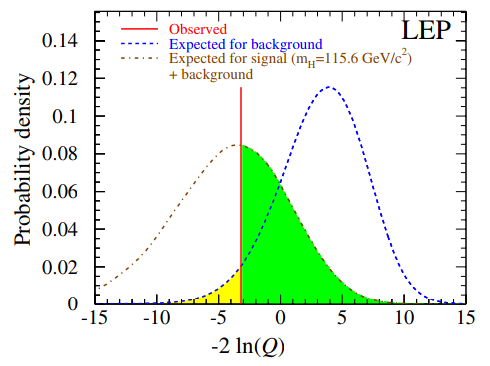
\includegraphics[width=0.5\textwidth]{figures/ci/cls.png}
% \caption{}
% \label{fig:ciClsNobs}
% \end{figure}

% CLs
% The PDF of $\Lambda(\nobs)$ is defined under both the B-only and S+B hypotheses.
The \emph{CLs method} is a statistical convention used in particle physics to compare hypotheses.
Taking first the PDF under the B-only hypothesis, $\Lambda(\nobs|\theta_0)$.
The integral of the test statistic $\Lambda(\nobs|\theta_0)$ above a given observed value of $\nobs$ defines the \emph{p-value}, $p_0$, of the observation.
This is the probability, according to the B-only hypothesis, to observe a value of the test statistic that is less likely than the actual observed value.
The p-value is illustrated in the shaded blue areas of the plots in Figure \ref{fig:ciCls}.
The complement of the p-value, shown as the unshaded region under the blue curve, defines the value $\clb\equiv1-p_0$.
An analogous value, $\clsb$, is defined for the likelihood ratio under the S+B hypothesis, using the PDF $\Lambda(\nobs|\theta_1)$.
The value $p_1$ is the defined as the integral of $\Lambda(\nobs|\theta_1)$ above the observed value, and $\clsb\equiv1-p_1$.
Finally, the ratio of these two values defines the arbitrarily named value $\cls\equiv \clsb/\clb$.
This ratio is interpreted as the confidence in the S+B hypothesis compared to the B-only hypothesis \cite{read}.

\subsection{Statistical Model}\label{sec:ciStatModel}

Each statistical question is answered through the comparison of B-only and S+B hypotheses.
Three related tests are performed;
\begin{enumerate}
    \item the background-only hypothesis versus a generic model-independent hypothesis of signal events;
    \item the background-only hypothesis versus a contact interaction hypothesis involving either lepton channel;
    \item the background-only hypothesis versus a contact interaction hypothesis involving both lepton channels.
\end{enumerate}
Each of these hypotheses is described by one of the following likelihood functions.
The likelihood converts the hypothesis into an expression of the probability to observe a yield in an SR.
In each case, a \emph{parameter of interest} (POI) is used to define the signal hypothesis.
For the model-independent hypothesis of a generic signal production, the POI is the number of signal events produced in the SR, $N_s$.
For the contact interaction model, the POI is the energy scale \lam. Different values of \lam correspond to different S+B hypotheses.
Figure \ref{fig:ciNSigInSr} shows that, in the case of CI models, the number of signal events produced is a function of \lam: $N_s(\lam)$.
Comparisons of the model-independent results with the CI results provide a useful cross-check.

The first likelihoods describe the background-only hypothesis and a hypothesis predicting some number of signal events, $N_s$, to be reconstructed in the SR.
In this model, the POI is $N_s$.
The PDFs of the number of events to observe in the SR for each hypothesis are given in Equations \ref{eqn:ciNullLikelihoodNSig} and \ref{eqn:ciAltLikelihoodNSig}.
\begin{flalign}
\text{PDF}_\text{b}(\vec{\theta}) =& \text{Pois}((1+\theta_\text{b})\times N_b) \times \text{Gaus}(\theta_\text{b},\sigma_\text{b}) \label{eqn:ciNullLikelihoodNSig}\\
\text{PDF}_\text{s+b}(\vec{\theta}) =& \text{Pois}(N_s+(1+\theta_\text{b})\times N_b) \times \text{Gaus}(\theta_\text{b},\sigma_\text{b}) \label{eqn:ciAltLikelihoodNSig}
\end{flalign}
The functions $\text{Pois}(N_\text{exp})$ are Poisson probability distributions with medians $N_\text{exp}$.
In this case, $N_\text{exp}=(1+\theta_\text{b})\times N_b$, where $N_b$ is the expected background in the SR from the extrapolation procedure.
The parameter $\theta_\text{b}$ is a nuisance parameter that is fit to the data and corresponds to the measured uncertainty on $N_b$.
The functions $\text{Gaus}(\theta_\text{b},\sigma_\text{b})$ are Gaussian constraints on the nuisance parameter $\theta_\text{b}$. These have means centered at $\theta_\text{b}=0$, and standard deviations $\sigma_\text{b}$.
For these PDFs, which are constructed to be agnostic as to the form of the signal model, the uncertainty $\sigma_\text{b}$ is the sum in quadrature of the extrapolation uncertainty and the ISS.

Next are the PDFs for hypotheses describing contact interactions, limited to individual lepton channels.
Equations \ref{eqn:ciNullLikelihood} and \ref{eqn:ciAltLikelihood} give the probability distributions for B-only and S+B hypotheses, respectively.
\begin{flalign}
\text{PDF}_\text{b}(\vec{\theta}) =& \text{Pois}((1+\theta_\text{b})\times N_b) \times \text{Gaus}(\theta_\text{b},\sigma_\text{b}) \label{eqn:ciNullLikelihood}\\
\text{PDF}_\text{s+b}(\vec{\theta}) =& \text{Pois}((1+\theta_\text{s})\times N_s(\Lambda)+(1+\theta_\text{b})\times N_b) \times \notag \\
                                          & \text{Gaus}(\theta_\text{b},\sigma_\text{b}) \times \text{Gaus}(\theta_\text{s},\sigma_\text{s}) \label{eqn:ciAltLikelihood}
\end{flalign}
The standard deviations of the Gaussian constraints correspond to the uncertainties described in Section \ref{sec:ciSyst}. 
$\sigma_\text{s}$ is the experimental uncertainty on the signal yield.
$\sigma_\text{b}$ is the total uncertainty on the background yield, which consists of the sum in quadrature of the extrapolation, ISS, and the function bias uncertainties.
Each of these numbers is given in Table \ref{tab:ciUncerts}.
The nuisance parameters are seen to modify the signal and background expectations in the Poisson function via $(1+\theta)$ terms.
In these models, the parameter of interest, \lam, is used to determine the number of signal events expected in the SR.
This is performed with a smooth interpolation between the generated CI shapes to provide $N_s(\lam)$.
For each of the four signals, a set of PDFs is constructed for each chirality combination, leading to 16 total models.

Last are the hypotheses dealing with CI models in both lepton channels.
These hypotheses predict signal production in both \ee and \mm channels.
For each constructive or destructive SRs, the observations in both \ee and \mm SRs are mutually independent.
Therefore the combined likelihood is the product of the individual likelihoods for each lepton channel corresponding to Equations \ref{eqn:ciNullLikelihood} and \ref{eqn:ciAltLikelihood}.
The observations in the constructive and destructive SRs of the same lepton channel are not mutually independent and therefore are not combined.
Consequently, for each interference pattern, the likelihoods of observations in the two leptonic SRs are combined to produce a total likelihood.
This is repeated for each chirality, resulting in eight pairs of hypotheses.

For each B-only and S+B ($\text{PDF}_\text{b}$ or $\text{PDF}_\text{s+b}$) PDF given here, a corresponding likelihood ($\mathcal{L}(\nobs|\theta_0)$ or $\mathcal{L}(\nobs|\theta_1)$) exists.
In this form, the likelihood expresses the probability of observing $\nobs$ events given some nuisance parameters $\theta$.

% Frequintist throw toys
It is helpful in computing \cls values to have PDF shapes, under both B-only and S+B hypotheses, for the likelihood ratio test statistic given in Equation \ref{eqn:ciLikelihoodTestStat}.
The PDF's shape is determined straightforwardly from the B-only and S+B PDF shapes with a frequentist Monte-Carlo procedure.
A number of pseudo-observations are generated from each hypothesis PDF ($\text{PDF}_\text{b}$ or $\text{PDF}_\text{s+b}$).
The nuisance parameters are allowed to vary corresponding to the width of their corresponding Gaussian constraint.
The number of observed events is sampled from the Poisson term.

The test statistic is calculated for each pseudo-observation.
This is simply a matter of fitting nuisance parameters of the appropriate likelihood ($\mathcal{L}(\nobs|\theta_0)$ or $\mathcal{L}(\nobs|\theta_1)$) to the pseudo-observation, and noting the probability of that observation.
This leads to distributions of the test statistic under each hypothesis, as shown in Figure \ref{fig:ciClsProfileLikelihood}.

\subsection{Significance test}\label{sec:ciSigTest}

\begin{figure}[h!]
\captionsetup[subfigure]{position=b}
\centering
\subfloat[][]{{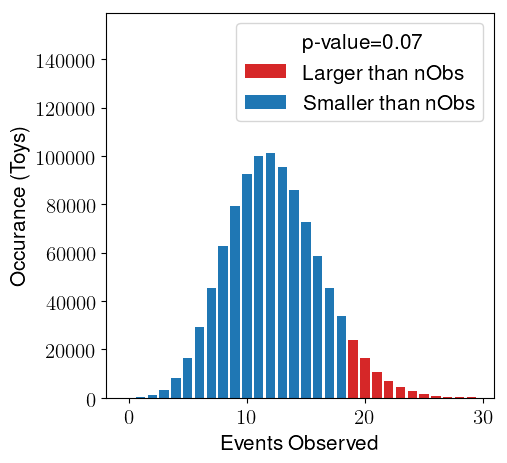
\includegraphics[width=0.24\textwidth]{figures/ci/nEventsTestStat/ee-const.png}}}
\subfloat[][]{{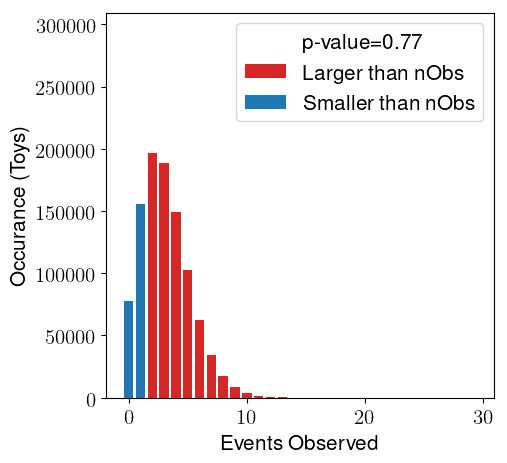
\includegraphics[width=0.24\textwidth]{figures/ci/nEventsTestStat/ee-dest.png}}}
\subfloat[][]{{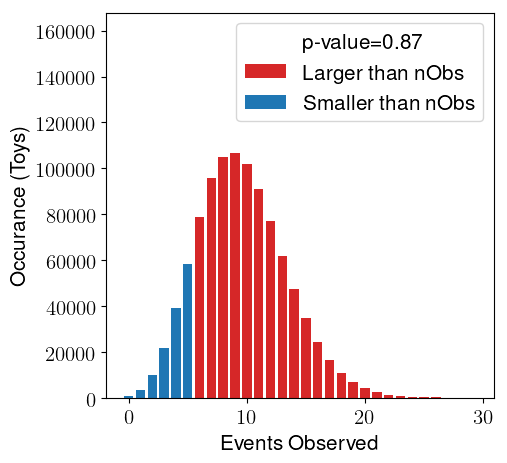
\includegraphics[width=0.24\textwidth]{figures/ci/nEventsTestStat/mm-const.png}}}
\subfloat[][]{{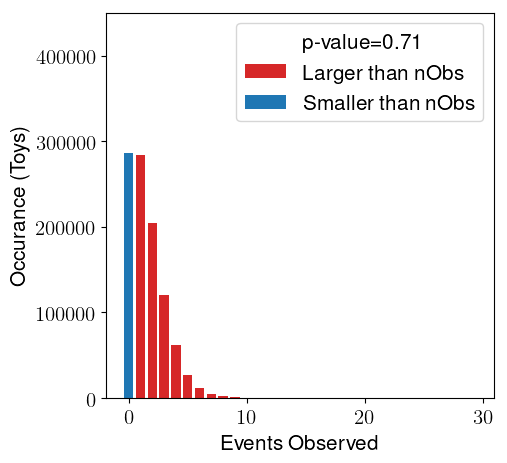
\includegraphics[width=0.24\textwidth]{figures/ci/nEventsTestStat/mm-dest.png}}}
\caption{Predictions of the B-only hypotheses estimated using ensembles of pseudo-experiments. The p-value is indicated in the shaded red region of the distribution. (a) and (b) show \ee constructive and destructive predictions, while (d) and (e) show \mm constructive and destructive predictions.}
\label{fig:ciSignificance}
\end{figure}

The significance of the data, given the background-only hypothesis, is evaluated by considering the p-value.
While it is possible to use the likelihood test statistic in Equation \ref{eqn:ciLikelihoodTestStat}, the signal dependence is undesirable.
Instead, the number of events yielded in the SR, \nobs, is used as the test statistic.
The corresponding p-value is the probability of observing a yield at least as large as that seen in data.
Figure \ref{fig:ciSignificance} shows the distributions of the event yields predicted by the background-only hypotheses in each SR.
The observed number of events is illustrated, and the integral corresponding to the p-value is highlighted.

The PDF distributions of \nobs is produced using a frequentist approach.
The shape is approximated with one hundred thousand pseudo-experiments drawn from the B-only hypothesis likelihood given in Equation \ref{eqn:ciNullLikelihood}.

Probabilities of observations are often cited in terms of standard deviations from the mean with respect to the normal distribution.
The background \emph{significance} of a p-value is defined as the inverse of the cumulative distribution function of the upper tail of the standard normal distribution.
This is illustrated for each SR in Figure \ref{fig:ciSignificance}.

\subsection{Limit test}\label{sec:ciLimitSetting}

Limit tests are a generalization of the significance test. %, where a set of signal+background hypotheses are rejected due to their incompatibility with the data.
In this context, the B-only hypothesis is taken to be the signal+background hypothesis, and the S+B hypothesis is defined as the background-only hypothesis $\text{PDF}_\text{b}$.
The hypothesis test then seeks to reject the signal+background hypothesis in favor of the background-only hypothesis due to their incompatibility with the observed data.
Values of the POI describe the set of signal+background hypotheses to be considered.
For the purpose of this analysis, this means the goal of the limit setting procedure is to find the limiting POI value that predicts the smallest non-rejected signal contribution to the SR.
This is done using a series of hypothesis tests scanned over a range of POI values. \footnote{An animated illustration of these scans may be found: \url{http://hg8i.com/thesis/likelihoods/}.}
This value is reported as the \emph{limit} on the POI.
Values of the POI that predict larger signal contributions to the SR describe excluded signal models, while values of the POI that predict fewer signal events in the SR remain admissible.

The compatibility of hypotheses with respect to the observation is measured using the \cls method.
The value of \cls plays a similar role as would a p-value.
For a particular value of the POI, if the \cls value exceeds 0.95, then the signal+background hypothesis is considered rejected, and the value of the POI is considered excluded.

There are two types of hyperparameters of the limit setting procedure.
First is the range and resolution of values to consider in a scan over the POI.
A broader range with finer resolution adds accuracy but also computational expense to the resulting limit.
This reaches a point of diminishing returns when the accuracy of the limit exceeds the second-order uncertainties on the systematics.
When the limiting value of the POI falls between steps in the POI scan, an interpolation is performed between the steps.
In general, 30 to 50 steps are sufficient for the results reported here.

The second type of hyperparameters defines the number of pseudo-observations, or toys, to calculate the PDF shapes for the test statistic.
The likelihood ratio (Equation \ref{eqn:ciLikelihoodTestStat}) serves as the test statistic for all limit setting.
The reliability of the results is quite sensitive to the number of toys.
Noting the log scale of Figure \ref{fig:ciClsProfileLikelihood} illustrates this point; many toys are needed to sample the tails of the likelihood distributions smoothly.
In this analysis, the limits were found to converge to a relative accuracy of $10^{-2}$ between one and two hundred thousand toys.
This 
For the results of this analysis, four hundred thousand toys were used for each POI step.
